\chapter{Einleitung}
\label{chap:einleitung}

In dieser Arbeit soll, mit Hilfe einer Simulation, untersucht werden, wie gut sich Kameras bei der Standortbestimmung in mobilen Roboter einsetzten lassen. Anlass dieser Arbeit war eine Anfrage der K�nstlergruppe \ac{BBM}, die schon bei mehreren Ausstellungen/Performances\footnote{unter Anderem:
  
  2000 Themenpark "Wissen" der Expo 2000 Hannover
  
  2010 Joybots  in der BMW-Welt 
  
  2012 EPKOT Experimental Prototype Killers of Tomorrow , Hannover
  
  siehe auch \url{ http://www.bbm.cfnt3.de}} mobile Roboter eingesetzt haben. Dabei interessierten sie sich f�r eine Lokalisierungsl�sung welche m�glichst ohne weitere spezial Hardware und geringem Installationsaufwand vor Ort auskommt. Der Ansatz der daraus entstand war: die Kameras, die bereits an jedem der Roboter verbaut waren, zu nutzen um markante Muster in der B�hneninstallation zu erkennen und gemeinsam mit den Odometrie-Daten zur Positionsberechnung zu verwenden. Dabei sollte ein Partikelfilter als Zustandssch�tzer verwendet werden. Zu der B�hneninstallation geh�ren gro�e Lichtw�nde, zu sehen auf Abbildung \ref{fig:RobotAndGuests} und \ref{fig:RobotAndLightwall}. Auf diese Lichtw�nde k�nnte ein hell/dunkel Bit-Muster angezeigt werden das es mit Hilfe geeigneter Bildverarbeitungsalgorithmen und mit den Kameras zu erkennen gilt.

  \begin{figure}[p]
    \centering
    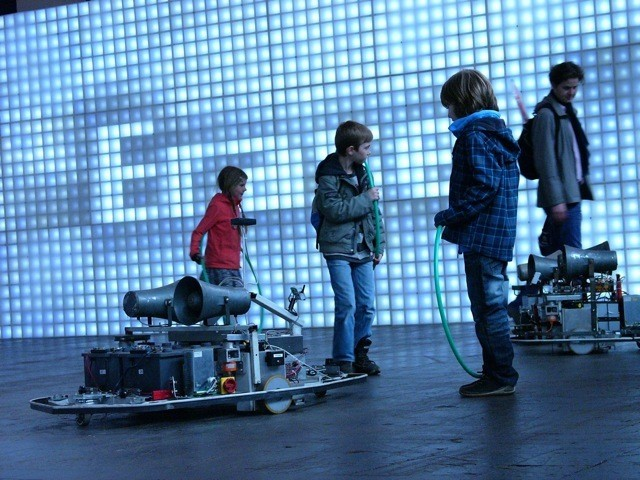
\includegraphics[width=\textwidth]{chapter1/roboterAndLightwallOnEPKOT2.png}
    \caption[Roboter und Besucher auf der EPKOT]{Roboter und Besucher auf der EPKOT Quelle: http://www.bbm.cfnt3.de}
    \label{fig:RobotAndGuests}
    \bigskip 
    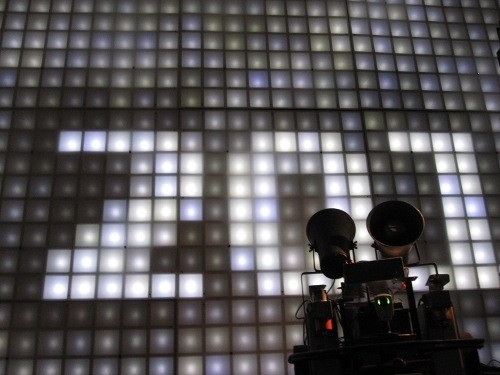
\includegraphics[width=\textwidth]{chapter1/roboterAndLightwallOnEPKOT.png}
    \caption[Roboter vor Lichtwand auf der EPKOT]{Roboter vor Lichtwand auf der EPKOT Quelle: http://www.bbm.cfnt3.de}
    \label{fig:RobotAndLightwall}
  \end{figure}
  
  \section{Ziel und Aufgabenstellung der Arbeit}
Im Rahmen dieser Arbeit soll eine Simulationsumgebung mit Hilfe geeigneter 3D-Visualisierungs Bibliotheken erstellt werden. Die in der Lage ist eine 3D-Szene der B�hne zu simulieren und Kamerabilder sowie Odometrie-Daten einer Roboterfahrt zu erzeugen. Au�erdem soll ein Lokalisationsalgorithmus entwickelt werden, der auf Grundlage dieser Daten die Position und Orientierung des Roboters auf der B�hne sch�tzen kann. Anschlie�end soll die Qualit�t dieser gesch�tzten Position beurteilt werden und m�gliche Fehlerquellen diskutiert werden.

  \section{Gliederung}
Die Arbeit wird im folgenden Kapitel eine �bersicht �ber g�ngige Lokalisationsverfahren sowie ihre Vor- und Nachteile geben. Anschlie�end wird die Simulations- und Lokalisationssoftware vorgestellt und deren Implementation erkl�rt und begr�ndet. In Kapitel \ref{chap:versuchsdurchfhrung} beginnt die Beschreibung verschiedene Versuche die zum Beurteilen der Lokalisationsergebnisse durchgef�hrt werden sollen. Danach werden die Ergebnisse dieser Versuche vorgestellt und in Kapitel \ref{chap:disskussiondermessergebnisse} Diskutiert.
Abschlie�end wird ein Ausblick zur m�glichen Anwendung dieses Verfahrens gegeben und ein Fazit gezogen.
  \begin{figure}[htbp]
    \centering
    \input{chapter1/loca_plot.tex}
    \caption{@@ PLATZHALTER @@}	
    \label{Sprungmarke1}
  \end{figure}